\chapter{Weryfikacja rozwiązania}

W celu weryfikacji poprawności działania zaimplementowanego systemu zostały
wykonane serie testów. System został przetestowany pod kątem sprawdzenia
podstawowych założeń projektowych tj. poprawności wykrywania anomali związanych
z natężeniem ruchu w obsługiwanej sieci oraz możliwości skalowania
aplikacji \textit{sdn\_epc} w celu zwiększenia wydajności systemu.
Przeprowadzenie testów wymagało przygotowania odpowiednich scenariuszy testowych,
zestawienia dedykowanych topolgi sieciowych oraz stworzenia rozwiązań
pozwalających na zebranie własciwych danych z testowanego systemu. Analiza
tychże wyników pozwoliła na stwierdzenie, czy i w jakim stopniu założenia
projektowe zostały spełnione. Niniejszy rozdział szczegółowo opisuje
poszczególne przypadki testowe oraz prezentuje analizę uzyskanych wyników.

\section{Test działania implementacji algorytmu}

Aby stwierdzić, czy zaimplementowany algorytm (rozdział \ref{algorithm} strona
\pageref{algorithm}) w aplikacji \textit{sdn\_epc} spełnia swoją rolę tzn.
pozwala wykryć atak DDoS w sieci SDN zostały przeanalizowane wartości entropii
obliczone za pomocą tegoż właśnie algorytmu w dwóch różnych przypadkach
testowych, z których każdy wykorzystywał nieco inną konfigurację testową
topologi sieciowej, jak również samej aplikacji \textit{sdn\_epc}. Przetestowane
zostały przypadki, gdy:  
\begin{enumerate}
  \item Ruch wygenerowany w sieci testowej był obsługiwany tylko przez jeden
    węzeł aplikacji \textit{sdn\_epc}.
  \item Ruch wygenerowanych w sieci testowej był obsługiwany przez wiele węzłów
    aplikacji \textit{sdn\_epc} działających w klastrze.
\end{enumerate}
Wykorzystanie takich właśnie przypadków testowych umożliwiło sprawdzenie
poprawności implementacji algorytmu zarówno w przypadku działania systemu jako
pojedynczy węzeł aplikacji \textit{sdn\_epc}, jak również w przypadku, gdy
system działał w klastrze. Drugi przypadek jest znacznie bardziej złożony,
ponieważ rozproszenie procesu obliczania algorytmu na wiele węzłów wprowadza
dodatkowe komplikacje, związane z synchronizacją stanu pomiędzy węzłami.

\subsection{Przypadek testowy z wykorzystaniem jednego węzła aplikacji
  \textit{sdn\_epc}} \label{entropy_one_node}

Schemat topologii sieciowej wykorzystanej w przypadku, gdy tylko jeden węzeł
aplikacji jest zaangażowany w przetwarzenie ruchu został przedstawiony na
Rys. \ref{fig:entropia_scheme}.

\begin{figure}[h]
\centering
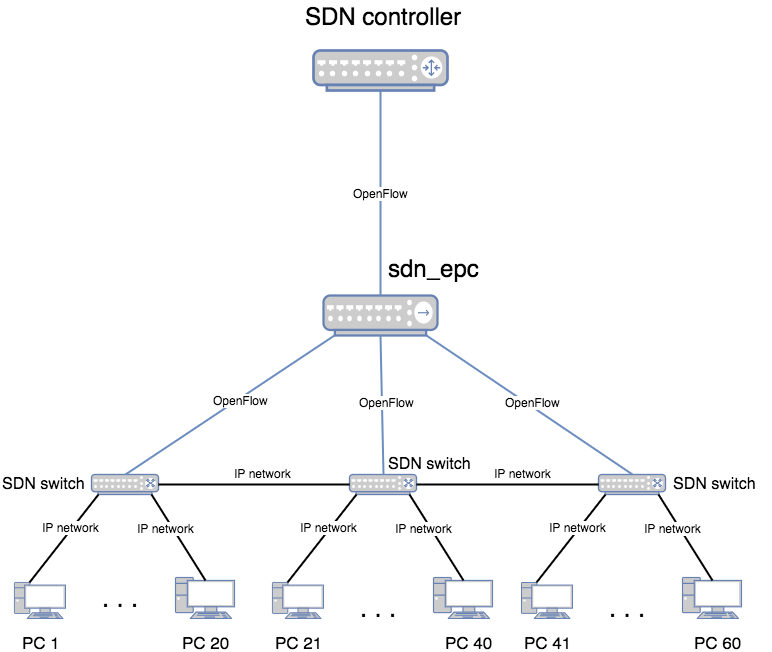
\includegraphics[width=\textwidth]{entropia_scheme}
\caption{Schemat topologii sieciowej z wykorzystaniem jednego węzła aplikacji
  \textit{sdn\_epc}}
\label{fig:entropia_scheme}
\end{figure}

W topologii przedstawionej na Rys. \ref{fig:entropia_scheme} wszystkie
przełączniki obsługujące ruch pomiędzy węzłami końcowymi (\textit{PC N})
komunikują się z kontrolerem (\textit{SDN controller}) poprzez jeden węzeł
aplikacji \textit{sdn\_epc}. Wykorzystując taką konfigurację sieci, tylko jeden
węzeł \textit{sdn\_epc} przetwarza wiadomości \mbox{\textit{PACKET\_IN}}
protokołu \textit{OpenFlow}, wymieniane pomiędzy poszczególnymi przełącznikami,
a kontrolerem, w celu obliczenia entropii pakietów przesyłanych w sieci.

Jeśli algorytm został poprawnie zaimplementowany to wartość entropii,
obliczonej za jego pomocą, powinna maleć wzraz ze spadkiem losowości pakietów
przesyłanych w sieci testowej. Innymi słowy, im więcej pakietów w sieci jest
adresowanych do jednego, konkretnego węzła końcowego, tym mniejsza będzie wartość
obliczonej entropii.

W celu sprawdzenia czy wspomiana zależność została spełniona, koniecznym było
zaprojektowanie odpowiedniego scenariusza testowego. Scenariusz ten opierał się
na środowisku testowym przedstawionym na Rys. \ref{fig:entropia_tech}.

\begin{figure}[h]
\centering
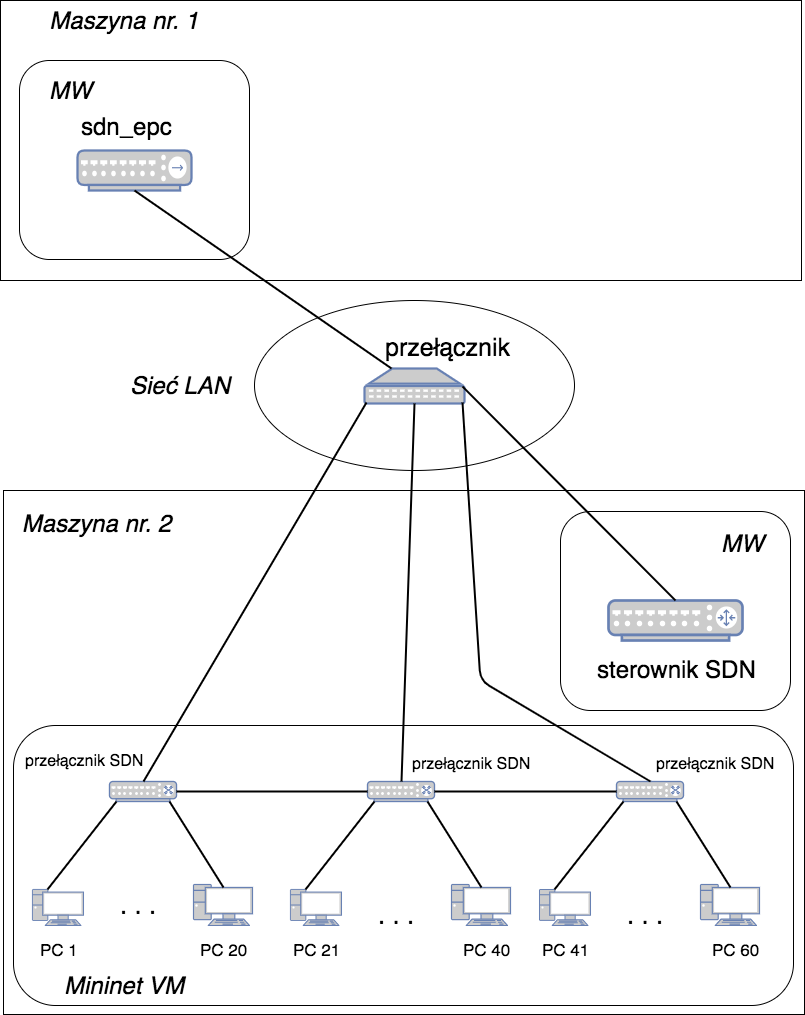
\includegraphics[height=11cm]{entropia_tech}
\caption{Środowisko testowe z wykorzystaniem jednego węzła aplikacji
  \textit{sdn\_epc}}
\label{fig:entropia_tech}
\end{figure}

Jak przedstawiono na Rys. \ref{fig:entropia_tech} toplogia sieciowa została
zestawiona z użyciem dwóch maszyn fizycznych, na których zostały zwirtualizowane
niezbędne komponenty testowe. Każdy z komponentów, za wyjątkiem przełącznika
sieci \textit{LAN} (\textit{switch}), został uruchomiony na dedykowanej maszynie
wirtualnej. Jako środowisko do wirtualizacji zostało wykorzystane oprogramowanie
\textit{VirtualBox \footnote{https://www.virtualbox.org}}. Maszyny wirtualne
komunikowały się ze sobą z wykorzystaniem sieci \textit{LAN}.

Przełączniki sieci SDN (\textit{SDN switch}) oraz węzły końcowe (\textit{PC
  N}) były emulowane na dedykowanej maszynie wirtualnej za pomocą oprogramowania
\textit{Mininet \footnote{http://mininet.org}}. Wykorzystane w teście
przełączniki to domyślne przełączniki używane przez oprogramowanie
\textit{Mininet}, które działają na bazie oprogramowania
\textit{Open vSwitch \footnote{http://openvswitch.org}} \cite{mininetwiki}.
\textit{SDN controller}, pełniący funkcję kontrolera w testowej topologii,
korzystał z oprogramowania zbudowanego z wykrzystaniem framework'a
\textit{Ryu \footnote{https://osrg.github.io/ryu}}. Maszyny wirtualne dedykowane
dla \textit{sdn\_epc} i \textit{SDN controller} działały pod kontrolą systemu
operacyjnego \textit{Ubuntu \footnote{https://www.ubuntu.com}}.

W celu poprawnego działania algorymu musi zostać spełnione założenie: dla
każdego nowego połączenia (adres źródłowy/docelowy, port źródłowy/docelowy oraz
protokół; na potrzeby ninejszej pracy wykorzystano tylko adres
docelowy/źródłowy) kontroler sieci SDN instaluje nowy przepływ w przełączniku
sieci SDN \cite{mainddosarticle}. Przy takim założeniu, każde nowe połączenie w
sieci wygeneruje wiadomość \textit{PACKET\_IN}, która następnie zostanie
przeanalizowana przez węzeł \textit{sdn\_epc}. Aby spełnić to założenie należało
zmodyfikować logikę przełącznika zaimplementowaną w kontrolerze. Modyfikacja
wymagała przeprogramowania \textit{Python}'owego skrytpu odpowiedzialnego za
implementację logiki przełącznika w oprogramowaniu kontrolera \cite{ryupage}.

Scenariusz testowy zakładał przeprowadzenie kilku prób, podczas których w sieci
były generowane ataki DDoS o różnej sile. Podczas każdej próby została zmierzona
średnia wartość entropii obliczonej za pomocą zaimplementowanego algorytmu.
Wykonane zostały cztery próby z atakami o sile odpowiednio: 0\%, 30\%, 60\% oraz
90\%. Siła każdego ataku została obliczona na podstawie wzoru
\ref{equ:ddos_power} \cite{mainddosarticle}

\begin{equation}
R = \frac{P_{a}}{P_{n}} \cdot 100\%
\label{equ:ddos_power}
\end{equation}
gdzie R oznacza siłę ataku, $P_{a}$ pakiety atakujące, natomiast $P_{n}$ pakiety
tła.

Pakiety tła rozumiane są jako pakiety
\textit{IP \footnote{https://tools.ietf.org/html/rfc791\#section-3.1}} wysyłane
do losowo wybranych węzłów końcowych w stałych odstępach czasowych. Pakiety
atakujące oznaczają pakiety \textit{IP}, które zawierają losowe adresy źródłowe
oraz są wysyłane do konkretnego węzła końcowego w 4-krotnie krótszych odstępach
czasowych niż pakiety tła. 

Podczas każdej próby wybrane węzły końcowe generowały pakiety tła oraz
pakiety atakujące (jeden węzeł generował jeden typ pakietów). Do generowania
pakietów została wykorzystana biblioteka języka \textit{Python} o nazwie
\textit{ Scapy \footnote{http://www.secdev.org/projects/scapy}}. Szczegółowe
dane opisujące każdą z prób zostały przedstawione w Tab. \ref{tab:entropy}.

\begin{table}[h!]
\centering
\begin{tabular}{ |c|c|c|c|c| } 
 \hline
 R & $P_{n}$ & $P_{a}$ & interwał $P_{n}$ & interwał $P_{a}$ \\
 \hline
 0\% & 3000 & 0 & 20ms & 5ms \\ 
 \hline
 30\% & 3000 & 900 & 20ms & 5ms \\ 
 \hline
 60\% & 3000 & 1800 & 20ms & 5ms \\ 
 \hline
 90\% & 3000 & 2700 & 20ms & 5ms \\ 
 \hline
\end{tabular}
\caption{Parametry prób testowych z wykorzystaniem jednego węzła aplikacji
  \textit{sdn\_epc}} 
\label{tab:entropy}
\end{table}

Warto zaznaczyć, że średnio 3,4\% wszystkich pakietów z danej próby nie dotarło
do aplikacji \textit{sdn\_epc}. Wydaje się, że nie powinno wpłynąć to znacząco
na uzyskane wyniki, jednak ze względu na fakt, że przeprowadzenie tego typu
testów wymaga znacznych zasobów obliczeniowych, do których dostęp nie jest
ogólnodostępny, wpływ wspomianego zjawiska nie został naukowo zbadany w
niniejszej pracy.

Na wykresie \ref{plot:entropy} przedstawiono średnią wartość entropii,
obliczonej przez aplikację \textit{sdn\_epc} przy użyciu zaimplementowanego w
niej algorytmu, dla poszczególnych prób testowych.

\begin{figure}[h]
\centering
\begin{tikzpicture}
\begin{axis}[
    xlabel={Siła ataku [\%]},
    ylabel={Średnia wartośc entropii},
    xmin=0, xmax=100,
    ymin=0.7, ymax=1.2,
    xtick={0,20,40,60,80,100},
    ytick={0.7,0.8,0.9,1,1.1,1.2},
    legend pos=outer north east,
    ymajorgrids=true,
    grid style=dashed,
]
 
\addplot[
    color=blue,
    mark=square,
    ]
    coordinates {
    (0,1.164)(30,1.025)(60,0.891)(90,0.748)
    };
    \legend{jeden węzeł \textit{sdn\_epc}}
 
\end{axis}
\end{tikzpicture}
\caption{Średnia wartość entropii w zależności od siły ataku DDoS}
\label{plot:entropy}
\end{figure}
\newpage

Zależność entropii od siły ataku, przedstawiona na wykresie \ref{plot:entropy},
jest taka, jak przewidywano. Wzraz ze wzrostem siły ataku wartość entropii
maleje, ponieważ im większa siła ataku, tym większy procent wszystkich pakietów
w sieci trafia do jednego, atakowanego, węzła końcowego. W związku z tym,
losowość poszczególnych pakietów spada, tym samym powodując spadek entropii
pakietów w sieci.

Bazując na przestawionych wynikach i ich analizie, można stwiedzić, że alogorytm
służacy do wykrywania ataku DDoS, został poprawnie zaimplementowany w aplikacji
\textit{sdn\_epc} i umożliwa wykrycie tego typu anomali. 

\subsection{Przypadek testowy z wykorzystaniem kilku węzłów aplikacji
  \textit{sdn\_epc} działających w klastrze} \label{entropy_multi_node}

Schemat topologii sieciowej wykorzystanej w przypadku, gdy kilka węzłów
aplikacji \textit{sdn\_epc} działających w klastrze obsługuje ruch w sieci
został zaprezentowany na Rys. \ref{fig:entropia_multi_scheme}.
\newpage

\begin{figure}[h]
\centering
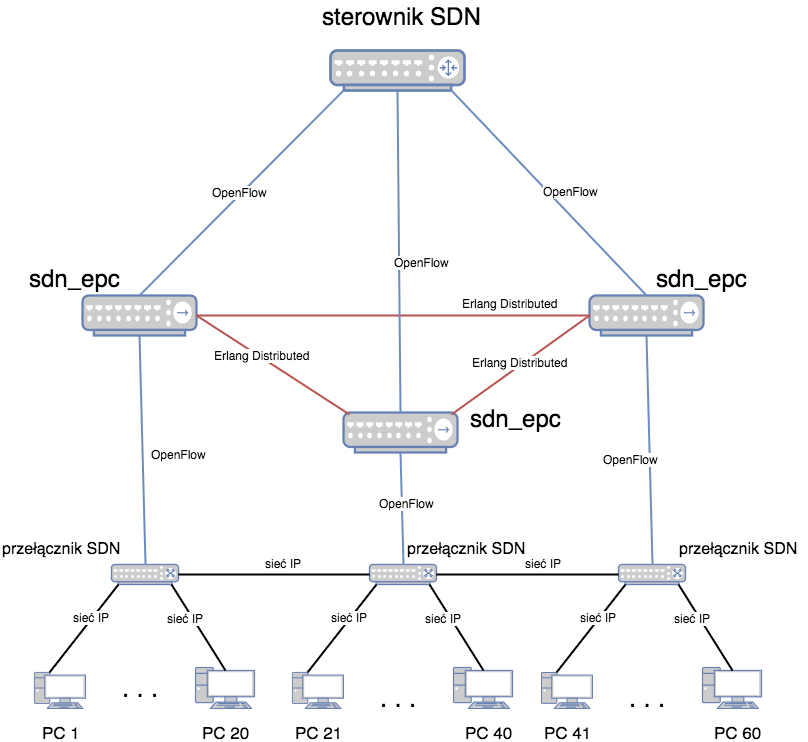
\includegraphics[width=\textwidth]{entropia_multi_scheme}
\caption{Schemat topologii sieciowej z wykorzystaniem trzech węzłów aplikacji
  \textit{sdn\_epc} działających w klastrze}
\label{fig:entropia_multi_scheme}
\end{figure}

Topologia przedstawiona na Rys. \ref{fig:entropia_multi_scheme} jest bardzo
podobna do przedstawionej na Rys. \ref{fig:entropia_scheme} na stronie
\pageref{fig:entropia_scheme}. W tym przypadku każdy przełącznik w sieci
komunikuje się z kontrolerem poprzez dedykowany węzeł aplikacji
\textit{sdn\_epc}, a więc w klastrze działa dokładnie tyle węzłów
\textit{sdn\_epc} ile jest przełączników w sieci. Każdy węzeł aplikacji obsłguje
tylko jeden przełącznik. Najważniejszą różnicą, względem przypadku, gdy tylko
jeden węzeł aplikacji obsługuje wszystkie przełączniki w sieci, jest 
rozproszenie procesu obliczania entropii na wiele węzłów \textit{sdn\_epc}.

W związku z tym, że rozposzenie procesu obliczania entropii na wiele węzłów,
wprowadziło szereg komplikacji, które należło uwzględnić, aby poprawnie ją
obliczyć, zostały przeprowadzene dokładnie takie same próby testowe, jak opisano
w sekcji \ref{entropy_one_node} ale z wykorzystaniem innej topologii testowej.
Przeprowadzenie bliźniaczych prób pozwoliło porównać wyniki, tj. wartości
entropii, w przypadku obliczania jej z użyciem jednego (patrz wykres
\ref{plot:entropy} strona \pageref{plot:entropy}) oraz kilku węzłów
\textit{sdn\_epc}. Takie porównanie pozwoliło ustalić, czy zaimplementowany
algorytm działa poprawnie również w przypadku rozproszenia procesu obliczania
entropii.

Środowisko przygotowane na potrzeby przeprowadzenia prób testowych, z
wykorzystaniem kilku węzłow \textit{sdn\_epc} przedstawiono na Rys.
\ref{fig:entropy_multi_tech}.

\begin{figure}[h]
\centering
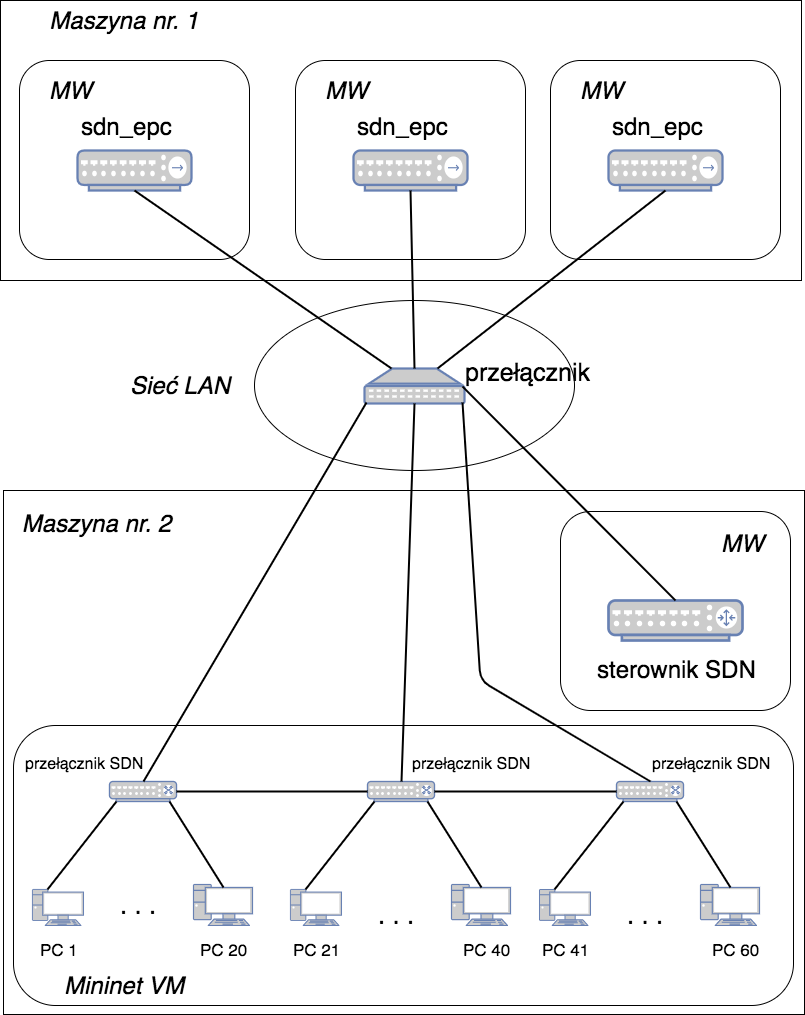
\includegraphics[height=11cm]{entropy_multi_tech}
\caption{Środowisko testowe z wykorzystaniem trzech węzłów aplikacji
  \textit{sdn\_epc} działających w klastrze}
\label{fig:entropy_multi_tech}
\end{figure}

Testowa topologia sieciowa przedstawiona na Rys. \ref{fig:entropy_multi_tech}
została zbudowana z takich samych komponentów i wykorzystując dokładnie takie
same rozwiązania i technologie jak przedstawiono na Rys. \ref{fig:entropia_tech}
strona \pageref{fig:entropia_tech} oraz opisano w sekcji \ref{entropy_one_node}.

W celu zmierzenia średniej wartości entropii z wykorzystaniem wielu węzłów
aplikacji \textit{sdn\_epc} przeprowadzono takie same próby testowe jak opisano
w Tab. \ref{tab:entropy} strona \pageref{tab:entropy}. Uzyskane wyniki zostały
przedstawione na wykresie \ref{plot:entropy_multi_node} wraz z wynikami
pozyskanymi podczas prób z wykorzystaniem jednego węzła \textit{sdn\_epc}, aby
umożliwić porównanie wyników otrzymanych z użyciem dwóch różnych topolgii
sieciowych.

\begin{figure}[h]
\centering
\begin{tikzpicture}
\begin{axis}[
    xlabel={Siła ataku [\%]},
    ylabel={Średnia wartośc entropii},
    xmin=0, xmax=100,
    ymin=0.7, ymax=1.2,
    xtick={0,20,40,60,80,100},
    ytick={0.7,0.8,0.9,1,1.1,1.2},
    legend pos=outer north east,
    ymajorgrids=true,
    grid style=dashed,
]

\addplot[
    color=blue,
    mark=square,
    ]
    coordinates {
    (0,1.164)(30,1.025)(60,0.891)(90,0.748)
    };
    \addlegendentry{jeden węzeł \textit{sdn\_epc}}

\addplot[
    color=red,
    mark=*,
    ]
    coordinates {
    (0,1.171)(30,1.027)(60,0.903)(90,0.746)
    };
    \addlegendentry{trzy węzły \textit{sdn\_epc}}

\end{axis}
\end{tikzpicture}
\caption{Średnia wartość entropii dla różnych konfiguracji testowych w
  zależności od siły ataku DDoS}
\label{plot:entropy_multi_node}
\end{figure}

Analizując wykres \ref{plot:entropy_multi_node} można zauważyć, że wartości
obliczonej entropii w obu przypadkach są niemal identyczne. Widoczne różnice
mogą być spowodowane przez straty pakietów w sieci (średnio w każdej próbie, z
wykorzystaniem topologii przedstawionej na Rys. \ref{fig:entropia_multi_scheme},
2,9\% wszystkich pakietów nie dotarło do węzła \textit{sdn\_epc}) oraz
niedoskonałością generatora losowego wykorzystanego do generowania adresów
docelowych dla pakietów \textit{IP} użytych do generowania ruchu podczas prób
testowych. Ze względu na ograniczenia techniczne, związane z dostępem do zasobów
obliczeniowych niezbędnych do przeprowadzenia testów, zjawiska te nie zostały
naukowo zbadane w niniejszej pracy. Jednakże różnice w wynikach są  na tyle
małe, że można uznać, iż zaimplementowany algorytm, służacy do wykrywania ataku
DDoS, działa poprawnie zarówno w systemie rozproszonym jak i z wykorzystaniem
jednego węzła \textit{sdn\_epc}.

\section{Test skalowalności horyzontalnej}

Celem weryfikacji skalowalności zaproponowanego rozwiązania zostały
przeprowadzone serie testów, podczas których zmierzono zużycie zasobów
obliczeniowych, a konkretnie czas zajętości procesora, wykorzystanych na
potrzeby przetwarzania ruchu sieciowego przez węzeł aplikacji \textit{sdn\_epc}.
Testy wykonano z wykorzystaniem dwóch różnych konfiguracji testowych:
\begin{enumerate}
  \item \label{tc:cluster_1} Ruch wygenerowany w sieci testowej był obsługiwany
    przez jeden węzeł aplikacji \textit{sdn\_epc} działający w klastrze.
  \item \label{tc:cluster_n} Ruch wygenerowany w sieci testowej był obsługiwany
    przez wiele węzłów aplikacji \textit{sdn\_epc} działających w klastrze.
\end{enumerate}

Porównanie średnich wartości czasu zajętości procesora pozwoliło stwierdzić,
czy dodanie kolejnych węzłów \textit{sdn\_epc} do klastra, celem rozłożenia
ruchu (obciążenia) na inne węzły, obniżyło zużycie zasobów przez pojedynczy
węzeł. Podczas każdej z prób testowych pomiary zostały przeprowadzone na tym
samym węźle aplikacji \textit{sdn\_epc}.

Schematy przedstawione na Rys. \ref{fig:cluster_scheme_single_node} oraz
Rys. \ref{fig:cluster_scheme_multi_node} prezentują odpowiednio przypadki
testowe opisane w Ad. \ref{tc:cluster_1} oraz Ad. \ref{tc:cluster_n}. Węzeł
na którym dokonano pomiarów został zaznaczony czerwonym okręgiem.
\newpage

\begin{figure}[h]
\centering
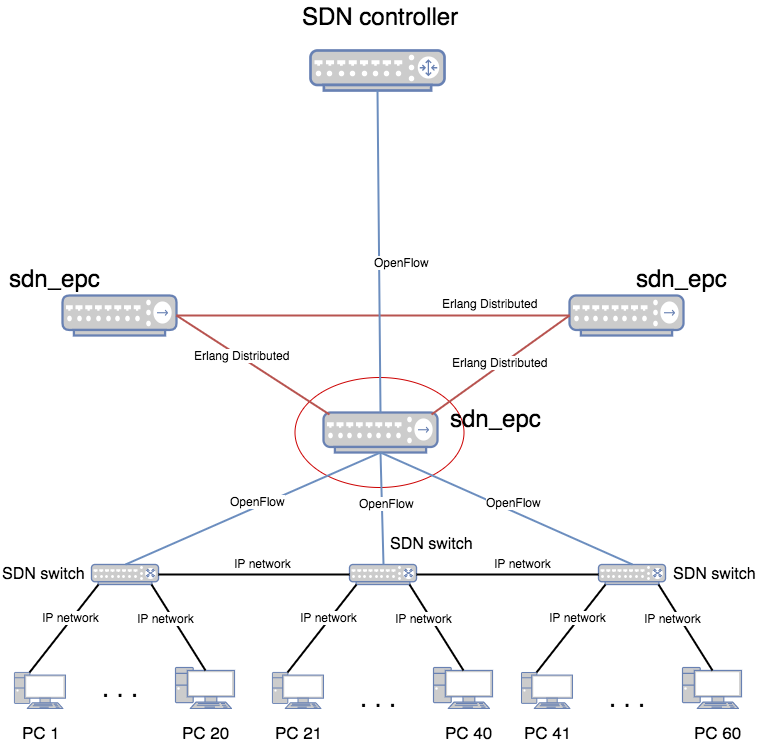
\includegraphics[width=\textwidth]{cluster_scheme_single_node}
\caption{Schemat topologii sieciowej z wykorzystaniem jednego węzła aplikacji
   \textit{sdn\_epc}, do obsługi ruchu sieciowego, działającego w klastrze}
\label{fig:cluster_scheme_single_node}
\end{figure}
\newpage

\begin{figure}[h]
\centering
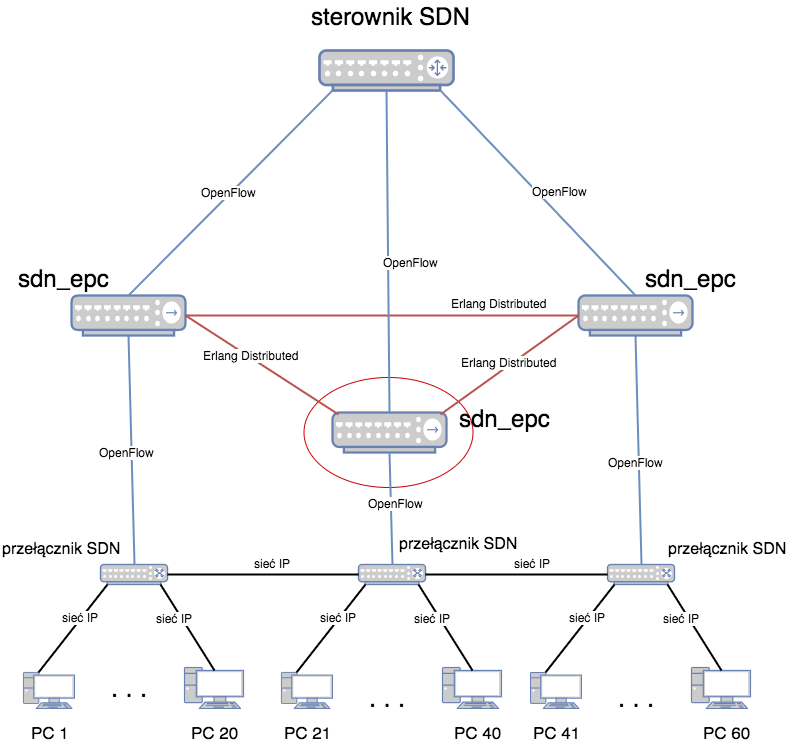
\includegraphics[width=\textwidth]{cluster_scheme_multi_node}
\caption{Schemat topologii sieciowej z wykorzystaniem trzech węzłów aplikacji
  \textit{sdn\_epc}, do obsługi ruchu sieciowego, działających w klastrze}
\label{fig:cluster_scheme_multi_node}
\end{figure}

Rozwiązanie przedstawione na Rys. \ref{fig:cluster_scheme_single_node}
wykorzystuje klaster węzłów \textit{sdn\_epc}, podczas gdy tylko jeden węzeł
jest zaangażowany w obsługę ruchu sieciowego. Takie rozwiązanie nie powinno być
wdrożone w jakimkolwiek systemie produkcyjnym, ponieważ budowanie klastra, w
którym używany jest tylko jeden węzeł w większości przypadków nie ma logicznego
uzasadnienia. Rozwiązanie to zostało wykorzystane na potrzeby niniejszej pracy
inżynierskiej tylko i wyłącznie z powodu niedoskonałości aplikacji
\textit{sdn\_epc}. W obecnej wersji aplikacji nie zostały dokonane żadne
optymalizacje związane z synchronizacją i dostępem do stanu pomiędzy węzłami. Z
powodu braku wspomnianych optymalizacji działanie aplikacji w klastrze wprowadza
znaczny narzut obliczeniowy. Użycie wymienionego wyżej rozwiązania pozwoliło
niejako ująć rzeczony narzut w pomiarach zużycia zasobów obliczeniowych dla
przypadku, gdy ruch sieciowy jest obsługiwany przez jeden węzeł
\textit{sdn\_epc}. Innymi słowy, różnica pomiędzy zmierzonym zużyciem zasobów
obliczeniowych dla wspominanych przypadków testowych nie zawiera wyż.wym.
narzutu. 

Architektura środowiska wykorzystanego na potrzeby testu jest dokładnie taka
sama jak przedstawiono na Rys. \ref{fig:entropy_multi_tech} strona
\pageref{fig:entropy_multi_tech} oraz opisano w sekcji \ref{entropy_multi_node}.
Wykorzystuje ona te same komponenty, rozwiązania oraz technologie jak te, które
opisano w wyż.wym. sekcji.

Scenariusz testowy, który wykorzystano podczas dwóch przeprowadzonych prób
testowych (Ad. \ref{tc:cluster_1} oraz Ad. \ref{tc:cluster_n} strona
\pageref{tc:cluster_1}) zakładał wykorzystanie odpowiednio logicznych topologii
sieciowych przedstawionych na Rys. \ref{fig:cluster_scheme_single_node} oraz
Rys. \ref{fig:cluster_scheme_multi_node}. Podczas każdej z prób wybrane węzły
końcowe wygenerowały 6000 pakietów tła (wyjaśnienie sekcja
\ref{entropy_multi_node}). Następnie na wybranym węźle aplikacji
\textit{sdn\_epc} (tym samym dla każdej próby) zmierzono średni czas zajętości 
procesora. Pomiarów dokonano z wykorzystaniem oprogramowania \textit{sysstat
  \footnote{http://sebastien.godard.pagesperso-orange.fr}}. Wyniki obu prób
przedstawiono na Rys. \ref{plot:cpu_usage}.

\begin{figure}[h]
\centering
\begin{tikzpicture}
\begin{axis}[
xbar,
width=10cm, height=3.5cm, enlargelimits=0.5,
xlabel={Średni czas zajętości procesora [\%]},
symbolic y coords={{1 węzeł sdn\_epc},{3 węzły sdn\_epc}},
ytick=data,
nodes near coords, nodes near coords align={horizontal},
]
\addplot coordinates {(35.30,{1 węzeł sdn\_epc}) (17.16,{3 węzły sdn\_epc})};
\end{axis}
\end{tikzpicture}
\caption{Średni czas zajętości procesora dla różnych konfiguracji testowych
  (rozmiarów klastra)}
\label{plot:cpu_usage}
\end{figure}

Na Rys. \ref{plot:cpu_usage} wyraźnie widać, że dla przypadku testowego, gdy
wygenerowany ruch sieciowy był obsługiwany przez 3 węzły \textit{sdn\_epc}
zużycie zasobów znacząco zmalało, względem próby, podczas której cały ruch
siecowy obsługiwał tylko jeden węzeł \textit{sdn\_epc}. Zużycie zasobów nie
zmalało dokładnie 3-krotnie, ponieważ działanie w aplikacji w klastrze wprowadza
dodatkowy narzut związany m.in. z rywalizacją węzłów o dostęp do stanu, który
jest niezbędny do ich poprawnego działania. Podsumowując wykres
\ref{plot:cpu_usage} dowodzi, że aplikację \textit{sdn\_epc} można skalować
horyzontalnie, co przynosi wymierne korzyści w postaci zwiększenia wydajności
całego rozwiązania, opisanego w niniejszej pracy.